% Created 2026-08-06 gio 14:50
% Intended LaTeX compiler: pdflatex
\documentclass[11pt]{article}
\usepackage[utf8]{inputenc}
\usepackage[T1]{fontenc}
\usepackage{graphicx}
\usepackage{longtable}
\usepackage{wrapfig}
\usepackage{rotating}
\usepackage[normalem]{ulem}
\usepackage{amsmath}
\usepackage{amssymb}
\usepackage{capt-of}
\usepackage{hyperref}
\usepackage[newfloat]{minted}
\author{Marco}
\date{\today}
\title{Elenco dei requisiti funzionali (versione rivista e completata)}
\hypersetup{
 pdfauthor={Marco},
 pdftitle={Elenco dei requisiti funzionali (versione rivista e completata)},
 pdfkeywords={},
 pdfsubject={},
 pdfcreator={Emacs 30.2 (Org mode 9.7.29)}, 
 pdflang={English}}
\begin{document}

\maketitle
\tableofcontents

\section{Perche' esiste questo file}
\label{sec:org943bd79}

Nella documentazione finale (\texttt{doc/documentazioneFinale/DocumentazioneDelSistemaMonitoraggioEGestioneDelTrafficoFerroviario.org},
sezione ``Elenco maggiomente formale dei requisiti'') l'elenco degli RF era stato buttato giu' di getto
all'inizio del progetto: due soli requisiti radice, RF01 (casi d'uso) e RF02 (correttezza del sistema
gestionale), con sotto i rami del dominio.

Quella lista adesso non regge piu' per tre motivi:

\begin{enumerate}
\item \textbf{e' rimasta indietro rispetto al codice}: nel frattempo sono stati implementati heartbeat,
watchdog, storicizzazione, andata/ritorno, autenticazione e TLS, e di tutto questo nella lista
non c'e' traccia;
\item \textbf{ha due voci sbagliate}, non solo incomplete: lo storico dichiarato ``non richiesto'' (il PDF del
prof lo chiede esplicitamente, ed e' pure implementato) e la frase sulla modifica della tratta
che dice il contrario di quello che intendeva;
\item \textbf{non distingue cio' che e' fatto da cio' che non lo e'}, e all'interrogazione questa e' proprio
la distinzione che conviene avere chiara: meglio dire ``questo requisito l'ho scritto e l'ho
implementato a meta', ecco dove si rompe'' che farsi trovare impreparati.
\end{enumerate}

Questo file quindi \textbf{sostituisce} quella lista. La documentazione finale puo' rimandare qui.
\section{Come si legge l'elenco}
\label{sec:org5c739bb}

Ogni requisito e' scritto con quattro informazioni:

\begin{description}
\item[{\textbf{enunciato}}] cosa il sistema deve fare, in una frase, al presente;
\item[{\textbf{origine}}] da dove viene il requisito. Tre possibilita':
\begin{itemize}
\item \texttt{PDF} = chiesto dal testo del prof (\texttt{doc/Progetto finale 2025\_26.pdf}),
\item \texttt{derivato} = non scritto nel PDF ma necessario perche' un requisito \texttt{PDF} stia in piedi,
\item \texttt{scelta} = decisione progettuale mia, il PDF lasciava liberta';
\end{itemize}
\item[{\textbf{stato}}] \texttt{IMPLEMENTATO}, \texttt{PARZIALE} (con la spiegazione di cosa manca), \texttt{FUORI AMBITO} (deciso
di non farlo, e si dice perche');
\item[{\textbf{dove}}] il punto del codice che lo realizza e la macchina a stati corrispondente nei diagrammi
(\texttt{T*} treno, \texttt{S*} stazione, \texttt{M*} centrale), cosi' il requisito e' navigabile fino alla riga.
\end{description}

La numerazione e' gerarchica e la gerarchia ha un significato preciso, lo stesso del grafo delle
dipendenze: \texttt{RF0X.Y} e' una \textbf{parte} di \texttt{RF0X} (decomposizione), mentre ``dipende da'' e' un'altra
relazione e viene scritta a parte. Sono due cose diverse e nel grafo hanno due tipi di freccia
diversi.
\section{Cosa e' stato corretto rispetto alla lista vecchia}
\label{sec:orgae8510d}

Riassunto delle modifiche, cosi' e' evidente cosa e' cambiato e non bisogna fare il diff a mano.
\subsection{Errori veri e propri}
\label{sec:org479ef90}

\begin{center}
\begin{tabular}{rlll}
\# & dove & com'era & com'e' adesso\\
\hline
1 & vecchio RF01 punto 4 & ``costruzione di uno storico (funzionalita' non richiesta)'' & RF01.5: il PDF la chiede (``gestire lo storico dei transiti'') ed e' implementata con sei tabelle \texttt{Storico*}\\
2 & vecchio RF02 modifica tratta & ``il treno \textbf{non} e' fuori dalla tratta il treno viene fermato in attesa di essere soppresso'' & RF02.5.1: e' il treno \textbf{fuori} dalla nuova tratta a essere fermato. Il ``non'' era di troppo e ribaltava la frase\\
3 & vecchio RF02 guasto treno & ``se il treno si guasta nella tratta si vuole che la \textbf{stazione} tratta' risultera' inusabile'' & RF02.1.2.2.2: e' la \textbf{tratta} a diventare inagibile, non la stazione\\
4 & scenari, Centrale & ``interrogare il database ogni 10 secondi per ogni tipo di visualizzazione'' & RF01.1.4: il tempo reale non e' polling del client, e' push su WebSocket piu' uno snapshot periodico da 10s lato server\\
\end{tabular}
\end{center}
\subsection{Requisiti che mancavano del tutto}
\label{sec:orgaaf6c2d}

Erano tutti gia' implementati, semplicemente non erano mai stati messi per iscritto:

\begin{itemize}
\item heartbeat stazione -> centrale e keepalive sensori -> stazione (RF02.3.2, RF02.3.3), che il PDF
chiede in modo esplicito nel paragrafo ``Guasto del Sensore/Stazione (Fail-Stop)'';
\item rilevazione automatica delle anomalie lato centrale, cioe' il watchdog (RF02.6): stazione muta e
treno fermo troppo a lungo fra due stazioni. Il secondo e' l'esempio testuale del PDF sotto
``Alerting'';
\item viaggio di andata e ritorno con inversione al capolinea (RF02.2.3), chiesto dal PDF (``sia
all'andata, che al ritorno'');
\item passaggi asimmetrici: il treno esce dalla stazione di partenza senza esserci entrato e entra al
capolinea senza uscirne (RF02.2.4), altro caso testuale del PDF;
\item comandi operativi del tecnico e dell'amministratore (RF01.4): invio della squadra di manutenzione,
presa in carico dell'allarme, soppressione del treno fermo in stazione;
\item autenticazione e permessi per ruolo (RF01.6 e RF04.1, RF04.2): il PDF chiede due tipologie di
utenti con poteri diversi, e la variante 2 permette il login tradizionale al posto di OAuth2;
\item cifratura dei canali (RF04.3): la variante 6 costa 5 punti se \textbf{non} si fa il TLS, quindi il fatto
di averlo fatto e' un requisito da dichiarare;
\item ecosistema di agenti, cioe' un processo per convoglio e uno per stazione (RF03.1): e' la
condizione che il PDF mette in maiuscolo per la sufficienza, e la variante 7 (accorpare le
stazioni in un servizio solo) costa altri 5 punti;
\item storicizzazione dei transiti e dei cambi di stato (RF02.7), che e' il lato dati di RF01.5.
\end{itemize}
\subsection{Requisiti che erano ottimisti}
\label{sec:org1b30ecb}

\begin{itemize}
\item RF02.5.2 (dopo la modifica della tratta il treno riprende dal punto in cui si trova) era dato per
fatto: in realta' e' \texttt{PARZIALE}, il digital twin ricarica l'itinerario ma riparte dalla prima
stazione. Sotto e' spiegato dove si rompe.
\end{itemize}
\section{RF01 - Casi d'uso dell'applicazione web}
\label{sec:org9e50fe3}

\textbf{Enunciato}: il sistema espone a tecnico e amministratore, attraverso un'unica applicazione web,
la situazione corrente della rete e i comandi previsti per il loro ruolo.

\textbf{Origine}: \texttt{PDF} (§3.C, ``questo server deve essere accessibile da due tipologie di utenti'').

\textbf{Nota di lettura}: RF01 non aggiunge logica di dominio, la \textbf{espone}. Per questo ogni suo ramo
scarica la dipendenza su RF02: se il dominio sotto e' sbagliato, la schermata mostra bene un dato
sbagliato.
\subsection{RF01.1 - Visualizzazione dei dati in tempo reale e corretti}
\label{sec:org4449077}

\subsubsection{RF01.1.1 - Mappa del traffico}
\label{sec:orgb2be27f}
\begin{itemize}
\item enunciato: la posizione dei convogli e' visibile su una mappa geografica, con la tratta percorsa
e lo stato del convoglio.
\item origine: \texttt{PDF} (visione d'insieme del traffico).
\item stato: \texttt{IMPLEMENTATO}.
\item dove: \texttt{ClientWebAppIntefacciaUtente/src/pages/TrafficMapPage.tsx}, alimentata da \texttt{M3} (telemetria)
e \texttt{M11} (websocket).
\end{itemize}
\subsubsection{RF01.1.2 - Elenco dei treni con posizione, stato e ritardo}
\label{sec:org158c9f7}
\begin{itemize}
\item enunciato: per ogni convoglio si vedono numero di convoglio, stazione o tratta su cui si trova,
stato (FERMO / IN\textsubscript{VIAGGIO} / EMERGENZA / SOPPRESSO), ritardo accumulato e passeggeri a bordo.
\item origine: \texttt{PDF} (il tecnico ``visualizza quali tratte segue un certo treno'').
\item stato: \texttt{IMPLEMENTATO}.
\item dove: \texttt{GET /api/treni}, \texttt{TrainsPage.tsx}; il dato nasce da \texttt{T8} e viene ingerito da \texttt{M3}.
\end{itemize}
\subsubsection{RF01.1.3 - Elenco delle stazioni con stato operativo e treni presenti}
\label{sec:org02f6b5a}
\begin{itemize}
\item enunciato: per ogni stazione si vedono lo stato (ONLINE / OFFLINE / GUASTA / MANUTENZIONE), i
treni attualmente fermi sui binari e quelli attesi in ingresso e in uscita.
\item origine: \texttt{PDF} (il tecnico ``visualizza quali treni ci si aspetta in ingresso e in uscita in una
certa stazione'').
\item stato: \texttt{IMPLEMENTATO}.
\item dove: \texttt{GET /api/stazioni}, \texttt{StationsPage.tsx}; stato di stazione = \texttt{M12}, presenze = \texttt{S11}.
\end{itemize}
\subsubsection{RF01.1.4 - Aggiornamento continuo senza ricaricare la pagina}
\label{sec:orgfe362ec}
\begin{itemize}
\item enunciato: le schermate si aggiornano da sole mentre l'operatore le guarda.
\item origine: \texttt{PDF} (obiettivo ``bassa latenza'': aggiornare la centrale in tempo reale).
\item stato: \texttt{IMPLEMENTATO}.
\item dove: WebSocket \texttt{/ws/realtime} (\texttt{RealtimeWebSocket}, \texttt{M11}) lato server, \texttt{websocketClient.ts} +
\texttt{useRealtimeUpdates.ts} lato client, con riconnessione automatica ogni 5s.
\item \textbf{correzione}: la vecchia frase ``interrogare il database ogni 10 secondi per ogni tipo di
visualizzazione'' descriveva un polling che non e' quello che fa il sistema. Il meccanismo e'
\textbf{push}: ogni evento rilevante (telemetria, transito, guasto, comando) viene spinto sul canale nel
momento in cui accade; i 10 secondi sono il periodo dello snapshot di riallineamento
(\texttt{FaultMonitor.broadcastSnapshot}), che serve a chi si e' appena collegato o ha perso messaggi,
non a fare da orologio dell'interfaccia.
\end{itemize}
\subsubsection{RF01.1.5 - Indicatori di sintesi}
\label{sec:org85deab7}
\begin{itemize}
\item enunciato: una dashboard riassume treni in circolazione, stazioni operative, guasti aperti e
ritardo medio.
\item origine: \texttt{scelta} (il PDF chiede una ``visione d'insieme'', la forma e' mia).
\item stato: \texttt{IMPLEMENTATO}.
\item dove: \texttt{GET /api/dashboard} -> \texttt{TrafficLogicEngine.kpiDashboard()}, \texttt{DashboardPage.tsx}.
\end{itemize}
\subsection{RF01.2 - Visualizzazione dei guasti}
\label{sec:org5adc338}

\subsubsection{RF01.2.1 - Elenco degli allarmi aperti}
\label{sec:org1060b67}
\begin{itemize}
\item enunciato: si vedono i guasti attivi con sorgente (quale stazione o quale treno), tipo, severita'
e istante di apertura.
\item origine: \texttt{PDF} (§ Alerting).
\item stato: \texttt{IMPLEMENTATO}.
\item dove: \texttt{GET /api/allarmi}, \texttt{AlertsPage.tsx}; il ciclo di vita e' \texttt{M7}.
\end{itemize}
\subsubsection{RF01.2.2 - Distinzione fra guasto segnalato e guasto dedotto}
\label{sec:orgf463999}
\begin{itemize}
\item enunciato: si distingue il guasto segnalato dal campo (un sensore lo ha dichiarato) da quello
dedotto dalla centrale (il nodo ha smesso di parlare).
\item origine: \texttt{derivato} da RF02.6: sono due guasti con cause diverse e vanno letti diversamente,
perche' il secondo puo' anche essere solo un problema di rete.
\item stato: \texttt{IMPLEMENTATO}.
\item dove: campo \texttt{sorgenteTipo} / creazione via \texttt{FaultMonitor.creaGuastoAutomatico} contro
\texttt{IngestionService.onAlert} (\texttt{M6} e \texttt{M8}).
\end{itemize}
\subsection{RF01.3 - Modifica dei dati riservata all'amministratore}
\label{sec:org5a46935}

\textbf{Enunciato del ramo}: la CRUD sull'anagrafica della rete e' permessa al solo amministratore; il
tecnico vede tutto ma non modifica nulla.

\textbf{Origine}: \texttt{PDF} (§3.C: l'amministratore ``puo' aggiungere ed eliminare tratte, puo' modificare le
stazioni attraversate dai treni'').
\subsubsection{RF01.3.1 - Stazioni}
\label{sec:org9ad6bee}
\begin{itemize}
\item stato: \texttt{IMPLEMENTATO} — \texttt{POST/PUT/DELETE /api/stazioni[/\{id\}]}, \texttt{StationEditorModal.tsx}.
\end{itemize}
\subsubsection{RF01.3.2 - Treni}
\label{sec:orgb89047c}
\begin{itemize}
\item stato: \texttt{IMPLEMENTATO} — \texttt{POST/PUT/DELETE /api/treni[/\{id\}]}, \texttt{TrainEditorModal.tsx}.
\end{itemize}
\subsubsection{RF01.3.3 - Tratte elementari (il segmento fra due stazioni)}
\label{sec:orgd66ea8b}
\begin{itemize}
\item stato: \texttt{IMPLEMENTATO} — \texttt{POST/PUT/DELETE /api/tratte-elementari[/\{id\}]},
\texttt{TrackSegmentEditorModal.tsx}.
\end{itemize}
\subsubsection{RF01.3.4 - Itinerari e assegnazione dei convogli}
\label{sec:org3aa7cf6}
\begin{itemize}
\item enunciato: l'amministratore compone l'itinerario come sequenza ordinata di stazioni con i tempi
di percorrenza, e ci assegna sopra i convogli.
\item stato: \texttt{IMPLEMENTATO} — \texttt{POST/PUT/DELETE /api/tratte[/\{id\}]}, \texttt{RouteEditorModal.tsx}.
\item dipende da: RF02.5 (la modifica deve restare corretta anche a treni gia' in marcia).
\end{itemize}
\subsubsection{RF01.3.5 - Integrita' referenziale sulle cancellazioni}
\label{sec:org4139114}
\begin{itemize}
\item enunciato: cancellare un'entita' non deve lasciare in giro righe orfane, e non deve essere
possibile se qualcosa la sta ancora usando.
\item origine: \texttt{derivato} (senza questo la ``correttezza'' di RF02 dura fino alla prima DELETE).
\item stato: \texttt{IMPLEMENTATO} — es. \texttt{DELETE /api/tratte-elementari/\{id\}} rifiuta se esistono transiti
storici su quella tratta; \texttt{DELETE /api/stazioni/\{id\}} ripulisce prima transiti e storici collegati.
\end{itemize}
\subsection{RF01.4 - Comandi operativi}
\label{sec:orge9f6ef4}

\textbf{Nota}: questo ramo mancava del tutto nella vecchia lista, dove i comandi comparivano solo come
accenno dentro ``gestione guasti'' della sezione scenari.
\subsubsection{RF01.4.1 - Invio della squadra di manutenzione}
\label{sec:org2bbdebb}
\begin{itemize}
\item enunciato: il tecnico manda gli operatori su una stazione guasta; la stazione passa in
MANUTENZIONE e i nodi di campo ne vengono avvisati.
\item origine: \texttt{PDF} (§3.A: ``un tecnico possa inviare operatori per risolvere immediatamente il
guasto''; §3.C: il tecnico ``ha il compito di mandare operatori per riparare una stazione'').
\item stato: \texttt{IMPLEMENTATO}.
\item dove: \texttt{POST /api/stazioni/\{id\}/manutenzione} -> alert \texttt{MAINTENANCE\_DISPATCHED} su \texttt{railway/alerts};
\texttt{M10} in uscita, \texttt{S9} in ricezione.
\end{itemize}
\subsubsection{RF01.4.2 - Presa in carico e chiusura di un allarme}
\label{sec:org98df4c8}
\begin{itemize}
\item enunciato: il tecnico dichiara risolto un guasto; il guasto viene chiuso, storicizzato e il campo
riceve il \texttt{RESOLVED} che sblocca i treni fermi.
\item origine: \texttt{PDF} (la centrale ``potra' attivare la procedura di ripristino'').
\item stato: \texttt{IMPLEMENTATO} — \texttt{POST /api/allarmi/\{id\}/risolvi}, \texttt{M7} + \texttt{M10}; lato treno e' \texttt{T9} che
aggiorna \texttt{T11}.
\end{itemize}
\subsubsection{RF01.4.3 - Soppressione di un convoglio fermo in stazione}
\label{sec:org9828190}
\begin{itemize}
\item enunciato: si sopprime una corsa; il convoglio passa in SOPPRESSO e smette di viaggiare.
\item origine: \texttt{PDF} (§3.C: l'amministratore ``(eventualmente) puo' sopprimere treni fermi in stazione'').
\item stato: \texttt{IMPLEMENTATO} — \texttt{POST /api/treni/\{id\}/sopprimi} -> alert \texttt{STOP} mirato sul convoglio.
\item \textbf{nota onesta}: nel PDF la soppressione e' attribuita all'amministratore, nel filtro di
autorizzazione l'ho messa fra i comandi operativi permessi anche al tecnico
(\texttt{FiltroAutorizzazione.richiedeAmministratore}, che lascia passare \texttt{/sopprimi}, \texttt{/risolvi} e
\texttt{/manutenzione} a entrambi i ruoli). E' una scelta discutibile: l'ho fatta perche' i tre comandi
sono la reazione a un'emergenza e il tecnico e' quello che sta davanti allo schermo quando
succede. Se all'interrogazione la si considera una deviazione dal testo, si stringe cambiando una
riga in quel metodo.
\end{itemize}
\subsection{RF01.5 - Consultazione dello storico}
\label{sec:org1e6611b}

\begin{itemize}
\item enunciato: sono consultabili i transiti passati, con treno, stazione, tratta, verso e istante.
\item origine: \texttt{PDF} (§3.C, Storage: ``gestire lo storico dei transiti'').
\item stato: \texttt{IMPLEMENTATO}.
\item dove: \texttt{GET /api/transiti} legge \texttt{StoricoTransito}; il dato viene scritto da \texttt{M5}.
\item \textbf{correzione}: nella lista vecchia questa voce era annotata ``funzionalita' non richiesta''. E'
sbagliato due volte: il PDF la chiede in modo esplicito, e nel frattempo e' stata implementata.
Il lato dati (piu' ampio di quello esposto) e' RF02.7.
\end{itemize}
\subsection{RF01.6 - Accesso al sistema}
\label{sec:org0a6beb1}

\begin{itemize}
\item enunciato: l'accesso alle funzionalita' richiede login; la sessione accompagna ogni chiamata
successiva e si chiude con il logout.
\item origine: \texttt{PDF} + variante 2 (utenti memorizzati sul server e autenticazione tradizionale al posto
di OAuth2, nessuna penalita').
\item stato: \texttt{IMPLEMENTATO} — \texttt{POST /api/auth/login} e \texttt{/logout} (\texttt{AuthController}), token di sessione
in \texttt{SessioniAttive}, \texttt{LoginPage.tsx} + \texttt{authStore.ts}. Macchina \texttt{M9}.
\item rimando: i dettagli di sicurezza stanno in RF04.
\end{itemize}
\section{RF02 - Correttezza del sistema gestionale}
\label{sec:orgd06a467}

\textbf{Enunciato}: lo stato che il sistema mostra e persiste corrisponde a quello che sta realmente
succedendo nella rete simulata, anche in presenza di guasti, disconnessioni e modifiche fatte a
sistema acceso.

\textbf{Origine}: \texttt{scelta} come formulazione, ma raccoglie gli obiettivi del PDF (affidabilita': ``i dati di
transito non vadano persi'').
\subsection{RF02.1 - Gestione dei guasti}
\label{sec:orgee5412f}

\subsubsection{RF02.1.1 - Guasto della stazione}
\label{sec:orgb12639e}

\begin{enumerate}
\item RF02.1.1.1 - Guasto temporaneo: perdita della connessione con la centrale
\label{sec:org217d1a9}

\begin{enumerate}
\item RF02.1.1.1.1 - Cache locale e reinvio in massa
\label{sec:org6a58afd}
\begin{itemize}
\item enunciato: mentre il collegamento e' giu', la stazione accumula in locale tutto cio' che produce
e lo rispedisce quando la connessione torna.
\item origine: \texttt{PDF} (§3.A: ``la stazione deve implementare un meccanismo di caching locale per
reinviare i dati una volta ripristinata la connessione'').
\item stato: \texttt{IMPLEMENTATO}.
\item dove: \texttt{Stazioni/.../LocalBuffer.java} + \texttt{S4} (connettivita' e store-and-forward), svuotamento
guidato da \texttt{S7}. Per la demo la caduta si simula con \texttt{POST /stazione/rete/offline} e
\texttt{/rete/online}.
\end{itemize}
\item RF02.1.1.1.2 - Ordine di consegna preservato
\label{sec:orge4fc913}
\begin{itemize}
\item enunciato: il reinvio rispetta l'ordine di generazione; se una singola consegna fallisce,
l'evento torna \textbf{in testa} alla coda e non in fondo.
\item origine: \texttt{derivato} (senza questo l'ordine entrata/uscita di uno stesso treno si puo' invertire e
lo storico dei transiti diventa incoerente: e' esattamente il dato che RF01.5 mostra).
\item stato: \texttt{IMPLEMENTATO} — \texttt{S5}, ciclo di vita dell'evento di stazione.
\end{itemize}
\end{enumerate}
\item RF02.1.1.2 - Guasto permanente: la stazione non e' percorribile
\label{sec:org67904bf}

\begin{enumerate}
\item RF02.1.1.2.1 - Il treno diretto alla stazione guasta si ferma
\label{sec:orge1d66f7}
\begin{itemize}
\item enunciato: se la prossima stazione dell'itinerario e' guasta, il convoglio non ci entra e resta
fermo dov'e'.
\item origine: \texttt{PDF} (§3.A: ``la stazione segnala il guasto a ogni treno che entra in stazione, il quale
non riparte fino a quando il guasto non e' ripristinato'').
\item stato: \texttt{IMPLEMENTATO} — \texttt{T9} riceve il \texttt{GUASTO}, \texttt{T11} tiene l'elenco delle stazioni guaste note
al convoglio, \texttt{T5} usa quell'elenco per trattenere la partenza.
\end{itemize}
\item RF02.1.1.2.2 - Riparte solo al ripristino
\label{sec:org6d3c4b8}
\begin{itemize}
\item enunciato: il convoglio riparte quando arriva il \texttt{RESOLVED} di quella stazione, non prima e non
per timeout.
\item origine: \texttt{PDF} (stessa frase).
\item stato: \texttt{IMPLEMENTATO} — \texttt{T9} rimuove la voce da \texttt{T11}, \texttt{T5} riprende dalla fase in cui era.
\end{itemize}
\item RF02.1.1.2.3 - Il blocco vale anche per chi e' gia' fermo li'
\label{sec:org0ff90a0}
\begin{itemize}
\item enunciato: un convoglio gia' fermo nella stazione che si guasta non riparte finche' il guasto e'
aperto.
\item origine: \texttt{derivato} (altrimenti il guasto bloccherebbe solo chi arriva dopo, e la stazione non
sarebbe davvero inagibile).
\item stato: \texttt{IMPLEMENTATO} — stesso meccanismo \texttt{T11} / \texttt{T5}: la condizione e' sulla \textbf{prossima} tappa,
che per un treno in sosta e' quella in cui si trova.
\end{itemize}
\end{enumerate}
\end{enumerate}
\subsubsection{RF02.1.2 - Guasto del treno}
\label{sec:orgbfe37e4}

\begin{enumerate}
\item RF02.1.2.1 - Il guasto viene memorizzato in centrale
\label{sec:orge1f62c4}
\begin{itemize}
\item enunciato: quando un convoglio si guasta, la centrale ne apre e persiste il guasto.
\item origine: \texttt{PDF} (§3.B: il treno segnala i guasti alla centrale).
\item stato: \texttt{IMPLEMENTATO} — sensore di bordo \texttt{POST /treno/sensore/guasto} (\texttt{T10}) -> alert MQTT
(\texttt{T9=/gateway) -> =M6} -> entita' \texttt{Guasto} (\texttt{M7}).
\end{itemize}
\item RF02.1.2.2 - Gestione delle conseguenze
\label{sec:org1ebf4a3}

\begin{enumerate}
\item RF02.1.2.2.1 - Treno guasto \textbf{in stazione} => stazione inagibile
\label{sec:org6c8502a}
\begin{itemize}
\item enunciato: se il convoglio si guasta mentre e' fermo in stazione, quella stazione diventa GUASTA.
\item origine: \texttt{PDF} (§3.A: ``un treno deragliato che inibisce l'uso di una certa stazione'').
\item stato: \texttt{IMPLEMENTATO} — la decisione e' presa in \texttt{M6} sulla base della posizione del convoglio.
\item dipende da: RF02.2.2.1 (sapere se il treno e' in stazione o in tratta).
\end{itemize}
\item RF02.1.2.2.2 - Treno guasto \textbf{in tratta} => tratta inagibile
\label{sec:orgd7de3dd}
\begin{itemize}
\item enunciato: se il convoglio si guasta fra due stazioni, e' la tratta a diventare inagibile.
\item origine: \texttt{PDF} (stessa frase, ``o di una particolare linea della stazione'').
\item stato: \texttt{IMPLEMENTATO} — stessa logica di \texttt{M6}.
\item \textbf{correzione}: la vecchia formulazione diceva ``si vuole che la \textbf{stazione} tratta' risultera'
inusabile'', che confonde le due entita'. Qui la stazione non c'entra: il treno e' fermo in mezzo.
\end{itemize}
\end{enumerate}
\end{enumerate}
\subsubsection{RF02.1.3 - Ciclo di vita del guasto}
\label{sec:org21d16f5}
\begin{itemize}
\item enunciato: un guasto ha uno stato (aperto, presa in carico, chiuso), un'assegnazione e una traccia
storica; non ci sono due guasti aperti sulla stessa sorgente per lo stesso motivo.
\item origine: \texttt{derivato} (senza l'unicita' il watchdog aprirebbe un guasto ogni 10 secondi).
\item stato: \texttt{IMPLEMENTATO} — \texttt{M7}; l'unicita' e' garantita da
\texttt{TrafficLogicEngine.getGuastoApertoPerSorgente}; le tracce sono \texttt{StoricoGuasto} e
\texttt{StoricoAssegnazioneGuasto}.
\end{itemize}
\subsubsection{RF02.1.4 - Chiusura automatica quando la causa rientra}
\label{sec:orgfa31e88}
\begin{itemize}
\item enunciato: se un guasto era stato aperto dal watchdog per silenzio del nodo, il ritorno del
battito lo chiude da solo, senza bisogno del tecnico.
\item origine: \texttt{derivato} (un guasto dedotto va disfatto dalla stessa deduzione che l'ha creato,
altrimenti la lista degli allarmi si riempie di falsi positivi che nessuno chiude).
\item stato: \texttt{IMPLEMENTATO} — \texttt{IngestionService.onHeartbeat} (\texttt{M4}).
\end{itemize}
\subsection{RF02.2 - Gestione dei treni}
\label{sec:org44158c3}

\subsubsection{RF02.2.1 - Gestione dei ritardi}
\label{sec:org38d8621}

\begin{enumerate}
\item RF02.2.1.1 - Il ritardo si accumula quando il treno e' fermo e dovrebbe circolare
\label{sec:orgfcc88a3}
\begin{itemize}
\item origine: \texttt{PDF} (§3.C, Processing: ``calcolo dei ritardi'').
\item stato: \texttt{IMPLEMENTATO} — \texttt{T5}: il contatore cresce mentre il convoglio e' trattenuto.
\end{itemize}
\begin{enumerate}
\item RF02.2.1.1.1 - Ritardo per guasto
\label{sec:orgc2d34f1}
\begin{itemize}
\item stato: \texttt{IMPLEMENTATO}. Dipende da RF02.1.
\end{itemize}
\item RF02.2.1.1.2 - Ritardo per ordine dell'amministratore
\label{sec:orgb944438}
\begin{itemize}
\item stato: \texttt{FUORI AMBITO}. Non e' chiesto dal PDF e non l'ho implementato: non esiste un comando
``rallenta questo treno''. Resta scritto qui perche' era nella lista originale e per dire
esplicitamente che e' una scelta e non una dimenticanza.
\end{itemize}
\end{enumerate}
\end{enumerate}
\subsubsection{RF02.2.2 - Servire le informazioni di stato del convoglio}
\label{sec:org0b9a301}

\begin{enumerate}
\item RF02.2.2.1 - Posizione: su quale tratta o in quale stazione si trova
\label{sec:orgadd29e5}
\begin{itemize}
\item origine: \texttt{PDF} (§ Stato Interno del digital twin: stazione precedente, prossima stazione).
\item stato: \texttt{IMPLEMENTATO} — \texttt{T5} (fase del viaggio) + \texttt{T8} (telemetria ogni 5s) -> \texttt{M3}.
\item \textbf{nota}: questo e' il \textbf{nodo a diamante} del grafo delle dipendenze. ``Dove si trova il treno'' e' il
predicato da cui dipendono la gestione dei guasti (stazione inagibile o tratta inagibile), la
modifica della tratta e il watchdog dei treni fermi. Togliendolo cadono sei requisiti insieme.
\end{itemize}
\item RF02.2.2.2 - Ritardo accumulato
\label{sec:org11aa48c}
\begin{itemize}
\item stato: \texttt{IMPLEMENTATO}. Dipende da RF02.2.1.
\end{itemize}
\item RF02.2.2.3 - Stato del convoglio
\label{sec:org549e9f7}
\begin{itemize}
\item enunciato: il convoglio dichiara come sta (FERMO, IN\textsubscript{VIAGGIO}, EMERGENZA, SOPPRESSO), che e' cosa
diversa da dove sta.
\item origine: \texttt{derivato} (servono due variabili ortogonali: un treno in emergenza resta nella fase di
viaggio in cui era, e quando l'emergenza rientra riprende da li').
\item stato: \texttt{IMPLEMENTATO} — \texttt{T6} lato treno, normalizzato in \texttt{M13} sulla colonna \texttt{Treni.stato}.
\end{itemize}
\item RF02.2.2.4 - Velocita' e passeggeri
\label{sec:org63d2802}
\begin{itemize}
\item origine: \texttt{scelta} (rendono la simulazione leggibile sulla mappa).
\item stato: \texttt{IMPLEMENTATO} — \texttt{T8}.
\end{itemize}
\end{enumerate}
\subsubsection{RF02.2.3 - Andata e ritorno sullo stesso itinerario}
\label{sec:org8668a7e}
\begin{itemize}
\item enunciato: raggiunto il capolinea il convoglio inverte la marcia e rifa' l'itinerario al
contrario, con sosta doppia al capolinea e tempo di percorrenza letto sulla tappa opposta.
\item origine: \texttt{PDF} (§3.C: ``il viaggio che ogni treno deve fare (elenco di stazioni) sia all'andata,
che al ritorno''; e la direzione A/R compare anche nella richiesta della prossima stazione).
\item stato: \texttt{IMPLEMENTATO} — \texttt{T7}.
\item \textbf{nuovo}: mancava del tutto nella lista vecchia, pur essendo una richiesta esplicita.
\end{itemize}
\subsubsection{RF02.2.4 - Passaggi asimmetrici in stazione}
\label{sec:orgd2f0a64}
\begin{itemize}
\item enunciato: un convoglio puo' uscire da una stazione senza esserci entrato (stazione di partenza) e
puo' entrare in una stazione senza uscirne (capolinea).
\item origine: \texttt{PDF} (§3.A, testuale: ``un treno puo' uscire da una stazione senza entrarvi [\ldots{}] oppure
entrare senza uscirvi'').
\item stato: \texttt{IMPLEMENTATO} — alla prima partenza \texttt{TrainJourneyEngine.avviaViaggio} non pubblica nessuna
ENTRATA, solo la USCITA a fine sosta; al capolinea la USCITA arriva solo dopo l'inversione.
\item \textbf{perche' conta}: e' il caso che rompe gli abbinamenti ingenui entrata/uscita nello storico dei
transiti. Chi conta le coppie deve sapere che le prime e le ultime sono spaiate per costruzione.
\end{itemize}
\subsection{RF02.3 - Gestione delle stazioni}
\label{sec:org66ec225}

\subsubsection{RF02.3.1 - Informazioni rese alla visualizzazione}
\label{sec:org649320c}
\begin{itemize}
\item enunciato: la stazione sa dire quali treni ha sui binari, chi e' entrato e quando, chi e' uscito e
quando.
\item origine: \texttt{PDF} (§3.A, funzionalita' del nodo stazione).
\item stato: \texttt{IMPLEMENTATO}.
\item dove: \texttt{S11} (presenza sui binari), esposto da \texttt{GET /stazione/treni}; il transito ufficiale verso
la centrale nasce in \texttt{S8} e viene ingerito da \texttt{M5}.
\item dipende da: RF02.1.1.1.1 — la cache che serve la visualizzazione \textbf{e' la stessa} nata per
sopravvivere alla disconnessione, non e' una seconda cache. Nella lista vecchia il legame non era
scritto e sembravano due cose diverse.
\end{itemize}
\subsubsection{RF02.3.2 - Heartbeat verso la centrale}
\label{sec:org073b952}
\begin{itemize}
\item enunciato: la stazione manda un battito periodico alla centrale; il suo silenzio e' il segnale che
la centrale usa per dedurne la caduta.
\item origine: \texttt{PDF} (§3.A, Rilevamento: ``si suggerisce un meccanismo di Heartbeat/Keepalive [\ldots{}] sia
tra Centrale e Stazioni'').
\item stato: \texttt{IMPLEMENTATO} — \texttt{HeartbeatGenerator} ogni 10s su \texttt{railway/station/\{id\}/heartbeat} (\texttt{S3}),
consumato da \texttt{M4}.
\item \textbf{nuovo}: mancava nella lista vecchia, pur essendo la meta' del meccanismo di RF02.6.1.
\end{itemize}
\subsubsection{RF02.3.3 - Keepalive dei sensori verso la stazione}
\label{sec:org154790b}
\begin{itemize}
\item enunciato: i sensori di binario mandano un keepalive alla stazione; se uno tace, la stazione lo
segnala come guasto alla centrale.
\item origine: \texttt{PDF} (stessa frase: ``sia tra Stazioni e relativi sensori. [\ldots{}] se una Stazione non
ricevesse Keep Alive da uno o piu' sensori, segnalerebbe lo stato di guasta alla Centrale'').
\item stato: \texttt{IMPLEMENTATO} — \texttt{POST /stazione/sensore/heartbeat} (\texttt{S6}), sorveglianza in \texttt{S7} (job da
10s), stato risultante in \texttt{S10}.
\item \textbf{nuovo}: mancava, ed e' il livello di heartbeat piu' facile da dimenticare perche' non passa dal
broker.
\end{itemize}
\subsubsection{RF02.3.4 - Stato operativo dichiarato dalla stazione}
\label{sec:orgf27b528}
\begin{itemize}
\item enunciato: la stazione dichiara di se' due soli stati, ONLINE e GUASTA.
\item origine: \texttt{derivato}.
\item stato: \texttt{IMPLEMENTATO} — \texttt{S10}.
\item \textbf{nota}: sono due e non quattro come nella cache della centrale (\texttt{M12}). OFFLINE e MANUTENZIONE la
stazione non li puo' conoscere di se' stessa: il primo e' una deduzione della centrale sul proprio
silenzio (una stazione che si crede offline avrebbe comunque il canale per dirlo, e allora non lo
e'), il secondo e' una decisione presa dal tecnico. Chi legge i due diagrammi in parallelo deve
sapere che descrivono lo stesso oggetto da due punti di vista con informazione diversa.
\end{itemize}
\subsection{RF02.4 - Validazione del nodo di campo}
\label{sec:orgab1bb2f}

\subsubsection{RF02.4.1 - L'ID dichiarato viene validato sul database centrale}
\label{sec:orgf1b1745}
\begin{itemize}
\item enunciato: un nodo (treno o stazione) che si avvia dichiara il proprio ID alla centrale; se l'ID
esiste a database il nodo entra nel sistema, altrimenti no.
\item origine: \texttt{scelta} (il PDF non lo chiede; l'ho aggiunto perche' senza, chiunque avvii un processo
con un ID inventato inquina la centrale con telemetria di un convoglio che non esiste).
\item stato: \texttt{IMPLEMENTATO} — richiesta e risposta su MQTT: \texttt{T2} / \texttt{S2} lato campo,
\texttt{ExistIdForEdge} e \texttt{ExistIdForEdgeStazione} lato centrale (\texttt{M2}).
\end{itemize}
\subsubsection{RF02.4.2 - Esito negativo: il processo non prosegue}
\label{sec:org066abb5}
\begin{itemize}
\item enunciato: se l'ID non e' riconosciuto il processo termina con codice di uscita 1, non resta
acceso a vuoto.
\item stato: \texttt{IMPLEMENTATO} — \texttt{TrainDatabaseValidator} / \texttt{StationDatabaseValidator}.
\end{itemize}
\subsubsection{RF02.4.3 - Dipendenza fattorizzata}
\label{sec:org9f472b0}
\begin{itemize}
\item Non e' un requisito a se': e' la regola di lettura del grafo. Senza RF02.4 nessun nodo entra nel
sistema, quindi non arriva nessun dato e cadono per intero RF02.1, RF02.2 e RF02.3. Per questo nel
grafo la freccia di dipendenza e' disegnata una volta sola sui tre rami invece che su ogni foglia.
\end{itemize}
\subsection{RF02.5 - Modifica della tratta a sistema acceso}
\label{sec:org20ced76}

\textbf{Origine}: \texttt{PDF} (§3.C: l'amministratore ``puo' modificare le stazioni attraversate dai treni'').
\subsubsection{RF02.5.1 - Treno \textbf{fuori} dalla nuova tratta: viene fermato in attesa di soppressione}
\label{sec:orgb8bf073}
\begin{itemize}
\item enunciato: se dopo la modifica il convoglio non e' piu' assegnato ad alcun itinerario, smette di
viaggiare e resta in attesa di essere soppresso.
\item stato: \texttt{IMPLEMENTATO} — \texttt{updateTratta} sgancia i treni non piu' in elenco e manda comunque a tutti
(vecchi e nuovi) l'evento \texttt{ITINERARIO\_AGGIORNATO}; il convoglio sganciato ricarica, riceve 404 da
\texttt{GET /api/treni/\{id\}/itinerario} e resta fermo riprovando ogni 15s (\texttt{T3}).
\item \textbf{correzione}: la vecchia frase era ``il treno \textbf{non} e' fuori dalla tratta il treno viene fermato in
attesa di essere soppresso''. Con quel ``non'' diceva l'opposto, ed era anche in contraddizione con
il grafo delle dipendenze, dove la stessa voce era gia' scritta giusta.
\item \textbf{nota di codice}: i treni da avvisare vanno letti \textbf{prima} di riassegnare le associazioni,
altrimenti quelli appena sganciati non risultano piu' dalla query e continuano a girare sulla
tratta vecchia senza saperlo. E' commentato in \texttt{RestApiGateway.updateTratta}.
\end{itemize}
\subsubsection{RF02.5.2 - Treno \textbf{dentro} la nuova tratta: la segue dal punto in cui si trova}
\label{sec:org0bf6e2e}
\begin{itemize}
\item enunciato: se il convoglio e' ancora assegnato, dovrebbe proseguire sul nuovo itinerario a partire
dalla posizione in cui la modifica lo ha colto.
\item stato: \texttt{PARZIALE}.
\item \textbf{cosa funziona}: la notifica arriva (\texttt{ITINERARIO\_AGGIORNATO} mirato sull'ID del convoglio, \texttt{T9}) e
l'itinerario viene ricaricato al tick successivo (\texttt{TrainJourneyEngine.tick} alza il flag,
\texttt{tentaCaricamentoItinerario} riscarica in REST).
\item \textbf{cosa non funziona}: la ricarica azzera \texttt{viaggioAvviato}, quindi \texttt{avviaViaggio()} riposiziona il
convoglio su \texttt{indiceStazione = 0} con \texttt{direzione = "andata"}. In pratica il treno \textbf{riparte dal
primo capolinea del nuovo itinerario}, non da dove si trovava. Se la modifica lo coglie a meta'
tratta, la posizione fa un salto.
\item \textbf{come si chiuderebbe}: dopo la ricarica, cercare nel nuovo itinerario la stazione che il convoglio
aveva appena lasciato (\texttt{stazioneCorrente}); se c'e', ripartire da quell'indice conservando
direzione e ritardo; se non c'e' piu', ricadere sul comportamento attuale. Sono una decina di
righe in \texttt{avviaViaggio}, ma preferisco dichiararlo qui piuttosto che scrivere che e' fatto.
\item dipende da: RF02.2.2.1.
\end{itemize}
\subsection{RF02.6 - Rilevazione automatica delle anomalie (watchdog)}
\label{sec:org4cd37d3}

\textbf{Enunciato del ramo}: la centrale deduce da sola le anomalie che i nodi di campo non possono
segnalare, prima fra tutte la propria caduta.

\textbf{Origine}: \texttt{PDF} (§3.A Fail-Stop: ``se una stazione smette di inviare dati alla Centrale Operativa,
quest'ultima non capirebbe se la stazione sia guasta o se i treni non transitano''; §3.C Alerting:
``generazione automatica di allarmi in caso di anomalie, es. treno fermo tra due stazioni per troppo
tempo'').

\textbf{Nuovo}: tutto questo ramo mancava nella lista vecchia.
\subsubsection{RF02.6.1 - Stazione muta oltre la soglia => OFFLINE e guasto automatico}
\label{sec:org40ff0fe}
\begin{itemize}
\item stato: \texttt{IMPLEMENTATO} — \texttt{FaultMonitor.controllaHeartbeat}, job ogni 10s, soglia
\texttt{fault.heartbeat.timeout.secondi} (30s di default). Macchina \texttt{M8}.
\item dipende da: RF02.3.2 (senza il battito non c'e' il silenzio da misurare).
\item si chiude da solo per RF02.1.4.
\end{itemize}
\subsubsection{RF02.6.2 - Treno fermo fuori stazione oltre la soglia => allarme automatico}
\label{sec:orgca2929c}
\begin{itemize}
\item stato: \texttt{IMPLEMENTATO} — \texttt{FaultMonitor.controllaTreniFermi}, soglia
\texttt{fault.treno.fermo.timeout.secondi} (90s di default).
\item dipende da: RF02.2.2.1 — ``fuori stazione'' e' un predicato sulla posizione, ed e' il motivo per cui
il nodo a diamante regge anche questo ramo.
\end{itemize}
\subsubsection{RF02.6.3 - Snapshot periodico verso la dashboard}
\label{sec:orgcf15ddc}
\begin{itemize}
\item enunciato: ogni 10 secondi la centrale spinge sul canale realtime una fotografia completa dello
stato.
\item origine: \texttt{derivato} (serve a riallineare chi si e' appena collegato o ha perso messaggi; e' il
vero significato dei ``10 secondi'' che nella lista vecchia erano scritti come polling).
\item stato: \texttt{IMPLEMENTATO} — \texttt{FaultMonitor.broadcastSnapshot} -> \texttt{M11}.
\end{itemize}
\subsection{RF02.7 - Storicizzazione}
\label{sec:org53d354f}

\begin{itemize}
\item enunciato: oltre allo stato corrente, il sistema conserva la traccia di cio' che e' successo:
transiti, cambi di stato dei treni e delle stazioni, guasti, assegnazioni degli operatori e
itinerari percorsi.
\item origine: \texttt{PDF} (§3.C Storage: stato attuale della linea \textbf{e} storico dei transiti).
\item stato: \texttt{IMPLEMENTATO} — entita' \texttt{StoricoTransito}, \texttt{StoricoStatoTreno}, \texttt{StoricoStatoStazione},
\texttt{StoricoGuasto}, \texttt{StoricoAssegnazioneGuasto}, \texttt{StoricoItinerario}.
\item \textbf{scelta di progetto}: lo stato \textbf{runtime} dei nodi vive in cache (\texttt{TrafficLogicEngine}), non a
database; a database ne resta la traccia storica. La cache si scrive a ogni frame di telemetria,
la riga storica solo \textbf{al cambio di stato} (\texttt{M3}). E' il motivo per cui un treno che manda 12 frame
al minuto non genera 12 righe al minuto.
\item e' il lato dati di RF01.5.
\end{itemize}
\section{RF03 - Ecosistema di agenti e comunicazione}
\label{sec:orgddbe3ab}

\textbf{Nuovo}: ramo assente dalla lista vecchia, che parlava solo di dominio. Serve perche' qui stanno le
condizioni architetturali che il PDF valuta a parte (e a punti).
\subsection{RF03.1 - Un processo per convoglio e un processo per stazione}
\label{sec:org2848417}
\begin{itemize}
\item enunciato: ogni treno e ogni stazione sono processi indipendenti, non oggetti dentro un
simulatore unico.
\item origine: \texttt{PDF} (§ Simulazione Dinamica: ``per rendere il progetto realistico (E OTTENERE LA
SUFFICIENZA), la simulazione non deve essere un unico blocco di codice, ma un ecosistema di
agenti''; inoltre la variante 7, che accorpa i servizi di monitoraggio delle stazioni in un unico
servizio, costa 5 punti e \textbf{non} e' stata presa).
\item stato: \texttt{IMPLEMENTATO} — moduli \texttt{Treni} (:8082) e \texttt{Stazioni} (:8081), N istanze ciascuno, ID passato
da argomento o property (\texttt{T1}, \texttt{S1}). I log per istanza stanno in \texttt{Stazioni/logs/}.
\end{itemize}
\subsection{RF03.2 - MQTT dal campo alla centrale}
\label{sec:org1627963}
\begin{itemize}
\item enunciato: la comunicazione fra nodi di campo e centrale passa dal broker, con topic gerarchici
per entita'.
\item origine: \texttt{PDF} (§4: MQTT dall'edge al core; la variante 4, stazioni che parlano REST, costa 5
punti e non e' stata presa).
\item stato: \texttt{IMPLEMENTATO}. Topic in uso:
\begin{center}
\begin{tabular}{llll}
topic & verso & contenuto & macchine\\
\hline
\texttt{railway/train/\{id\}/validation} & treno -> centrale & richiesta di validazione dell'ID & T2 -> M2\\
\texttt{railway/train/\{id\}/validation-response} & centrale -> treno & esito & M2 -> T2\\
\texttt{railway/station/\{id\}/validation} & staz. -> centrale & richiesta di validazione dell'ID & S2 -> M2\\
\texttt{railway/station/\{id\}/validation-response} & centrale -> staz. & esito & M2 -> S2\\
\texttt{railway/train/\{id\}/telemetry} & treno -> centrale & frame ogni 5s: posizione, stato, ritardo & T8 -> M3\\
\texttt{railway/train/\{id\}/passaggio} & treno -> tutti & ENTRATA / USCITA dichiarata dal convoglio & T-gw -> S8, M5\\
\texttt{railway/station/\{id\}/transit} & staz. -> centrale & transito ufficiale rilevato dai sensori & S8 -> M5\\
\texttt{railway/station/\{id\}/heartbeat} & staz. -> centrale & battito ogni 10s & S3 -> M4\\
\texttt{railway/alerts} & condiviso & GUASTO, RESOLVED, STOP, MAINTENANCE\textsubscript{DISPATCHED}, ITINERARIO\textsubscript{AGGIORNATO} & M6, M10, T9, S9\\
\end{tabular}
\end{center}
\end{itemize}
\subsection{RF03.3 - Un solo passaggio fisico, due strade indipendenti}
\label{sec:org7cc4225}
\begin{itemize}
\item enunciato: lo stesso transito arriva alla centrale per due vie: dal sensore di terra (che scrive
il transito storico) e dal convoglio (che aggiorna posizione e prossima stazione). Le due vie non
si sostituiscono a vicenda.
\item origine: \texttt{derivato} dal modello del PDF, dove il treno ``si presenta ai sensori'' e il sensore
``avverte la stazione, la quale inoltra il pacchetto dati alla Centrale''.
\item stato: \texttt{IMPLEMENTATO} — \texttt{IngestionService.onTransit} e \texttt{onPassaggio} (\texttt{M5}).
\item \textbf{nota}: e' il punto in cui e' piu' facile fare confusione durante l'interrogazione. La domanda
giusta e' ``perche' due?'': perche' il sensore e' la fonte di verita' per lo storico (esiste anche
se il treno tace) e il convoglio e' la fonte di verita' per la posizione (la sa prima e meglio del
sensore). Se ne togliessi una perderei o lo storico o il tempo reale.
\end{itemize}
\subsection{RF03.4 - REST dai sensori al nodo di campo}
\label{sec:org12c8026}
\begin{itemize}
\item enunciato: i sensori non toccano il modello del nodo: parlano solo attraverso le API REST che il
nodo espone.
\item origine: \texttt{scelta} (decisione di progetto documentata nel contratto di integrazione; il PDF lascia
liberta' sul collegamento sensore-nodo).
\item stato: \texttt{IMPLEMENTATO}.
\begin{itemize}
\item stazione (:8081, \texttt{StationIngestion}, \texttt{S6}): \texttt{POST /stazione/sensore/treno},
\texttt{/sensore/guasto}, \texttt{/sensore/heartbeat}, \texttt{/rete/offline}, \texttt{/rete/online};
\texttt{GET /stazione/info}, \texttt{/stato}, \texttt{/buffer}, \texttt{/treni};
\item treno (:8082, \texttt{TrainIngestion}, \texttt{T10}): \texttt{POST /treno/sensore/guasto}, \texttt{/sensore/passaggio},
\texttt{/tratta}; \texttt{GET /treno/info}, \texttt{/stato}, \texttt{/viaggio}, \texttt{/tratta}.
\end{itemize}
\item \textbf{perche' cosi'}: tenere i sensori fuori dal modello significa che la stessa macchina a stati vale
sia con la console interattiva della demo sia con un chiamante esterno, senza percorsi di codice
alternativi.
\end{itemize}
\subsection{RF03.5 - Itinerario e prossima stazione serviti dalla centrale}
\label{sec:org273bb44}
\begin{itemize}
\item enunciato: il convoglio scarica dalla centrale l'itinerario completo all'avvio; in piu' la
centrale sa rispondere alla domanda ``data la coppia treno + stazione attuale + direzione, qual e'
la prossima stazione?''.
\item origine: \texttt{PDF} (§ Simulazione Dinamica: entrambe le opzioni, tabella precaricata in memoria
\textbf{oppure} prossima stazione chiesta di volta in volta).
\item stato: \texttt{IMPLEMENTATO} — \texttt{GET /api/treni/\{id\}/itinerario} (\texttt{T3} -> \texttt{M10}) e
\texttt{GET /api/prossima-stazione}. Il motore usa la tabella precaricata; l'endpoint puntuale resta
disponibile per l'altra modalita'.
\item \textbf{nota}: sono le due sole GET che il filtro di autorizzazione lascia aperte, perche' i processi di
campo non fanno login (vedi RF04.2).
\end{itemize}
\section{RF04 - Sicurezza degli accessi e dei canali}
\label{sec:org03fcd72}

\textbf{Nuovo}: ramo assente dalla lista vecchia. Ci sono dentro punti di valutazione espliciti.
\subsection{RF04.1 - Autenticazione tradizionale}
\label{sec:org7030046}
\begin{itemize}
\item enunciato: gli utenti sono memorizzati sul server; l'accesso avviene con login e password e
produce un token di sessione.
\item origine: \texttt{PDF} variante 2 (esplicitamente ammessa al posto di OAuth2, \textbf{nessuna penalizzazione}).
\item stato: \texttt{IMPLEMENTATO} — entita' \texttt{Utente}, \texttt{AuthController}, \texttt{SessioniAttive} (\texttt{M9}).
\end{itemize}
\subsection{RF04.2 - Autorizzazione per ruolo}
\label{sec:org8868820}
\begin{itemize}
\item enunciato: ogni chiamata sotto \texttt{/api} porta il token; le letture sono permesse a entrambi i ruoli,
la CRUD sull'anagrafica al solo amministratore.
\item origine: \texttt{PDF} (due tipologie di utenti con poteri diversi).
\item stato: \texttt{IMPLEMENTATO} — \texttt{FiltroAutorizzazione}, filtro JAX-RS a priorita' di autenticazione.
\item eccezioni dichiarate, ognuna con il suo motivo:
\begin{itemize}
\item \texttt{POST /api/auth/login} pubblica: e' li' che si ottiene il token;
\item le \texttt{OPTIONS} passano: la preflight del browser non porta header applicativi e senza questo il
CORS fallisce prima della chiamata vera;
\item le due GET di RF03.5 restano aperte: i processi Treno e Stazione non fanno login, la loro
``autenticazione'' e' la validazione dell'ID di RF02.4. Sono due sole letture e nessuna scrittura.
\end{itemize}
\item \textbf{nota onesta}: prima la distinzione fra i due ruoli era solo grafica, cioe' il frontend nascondeva
i pulsanti ma chiunque poteva cancellare un treno con un \texttt{curl}. Il filtro nasce per chiudere
proprio quel buco, ed e' il tipo di domanda che vale la pena aspettarsi.
\end{itemize}
\subsection{RF04.3 - Canali cifrati}
\label{sec:org3cdd9f9}
\begin{itemize}
\item enunciato: tutti i canali (MQTT verso il broker e HTTP verso la centrale) possono girare cifrati.
\item origine: \texttt{PDF} variante 6 — \textbf{non} implementare TLS costa 5 punti, quindi implementarlo e' un
requisito da dichiarare.
\item stato: \texttt{IMPLEMENTATO} come profilo — profilo Quarkus \texttt{\%tls} su tutti e tre i moduli, MQTT su 8883
con truststore PEM, HTTPS della centrale su 8444; certificati generati da
\texttt{BrokerMosquitto/tls/gen-certs.sh}. Si attiva con \texttt{-Dquarkus.profile=tls}.
\item \textbf{attenzione}: sotto profilo TLS \textbf{ogni} canale deve avere \texttt{ssl=true}. Un solo canale dimenticato
apre una socket in chiaro su un listener TLS: l'handshake fallisce e il sintomo che si vede e' un
nodo che non valida l'ID, non un errore di certificato. E' il motivo per cui negli
\texttt{application.properties} gli override \texttt{\%tls.*} sono ripetuti canale per canale invece che
raggruppati.
\end{itemize}
\section{Grafo delle dipendenze aggiornato}
\label{sec:orgcf9d7b6}

Stesse convenzioni del grafo precedente (\texttt{00\_grafo\_dipendenze\_requisiti.puml}): linea piena \texttt{*-{}-{}}
per la decomposizione, freccia tratteggiata \texttt{..>} per la dipendenza, cioe' ``togliendo il bersaglio
il requisito non e' piu' soddisfacibile'' (test di eliminazione). Il file \texttt{00\_} descrive la lista
vecchia ed e' quindi superato da questo.

Per non riempire il disegno di frecce ripetute vale la regola gia' usata: se tutte le parti di A
dipendono da D, la freccia si mette una volta sola su A.

\begin{center}
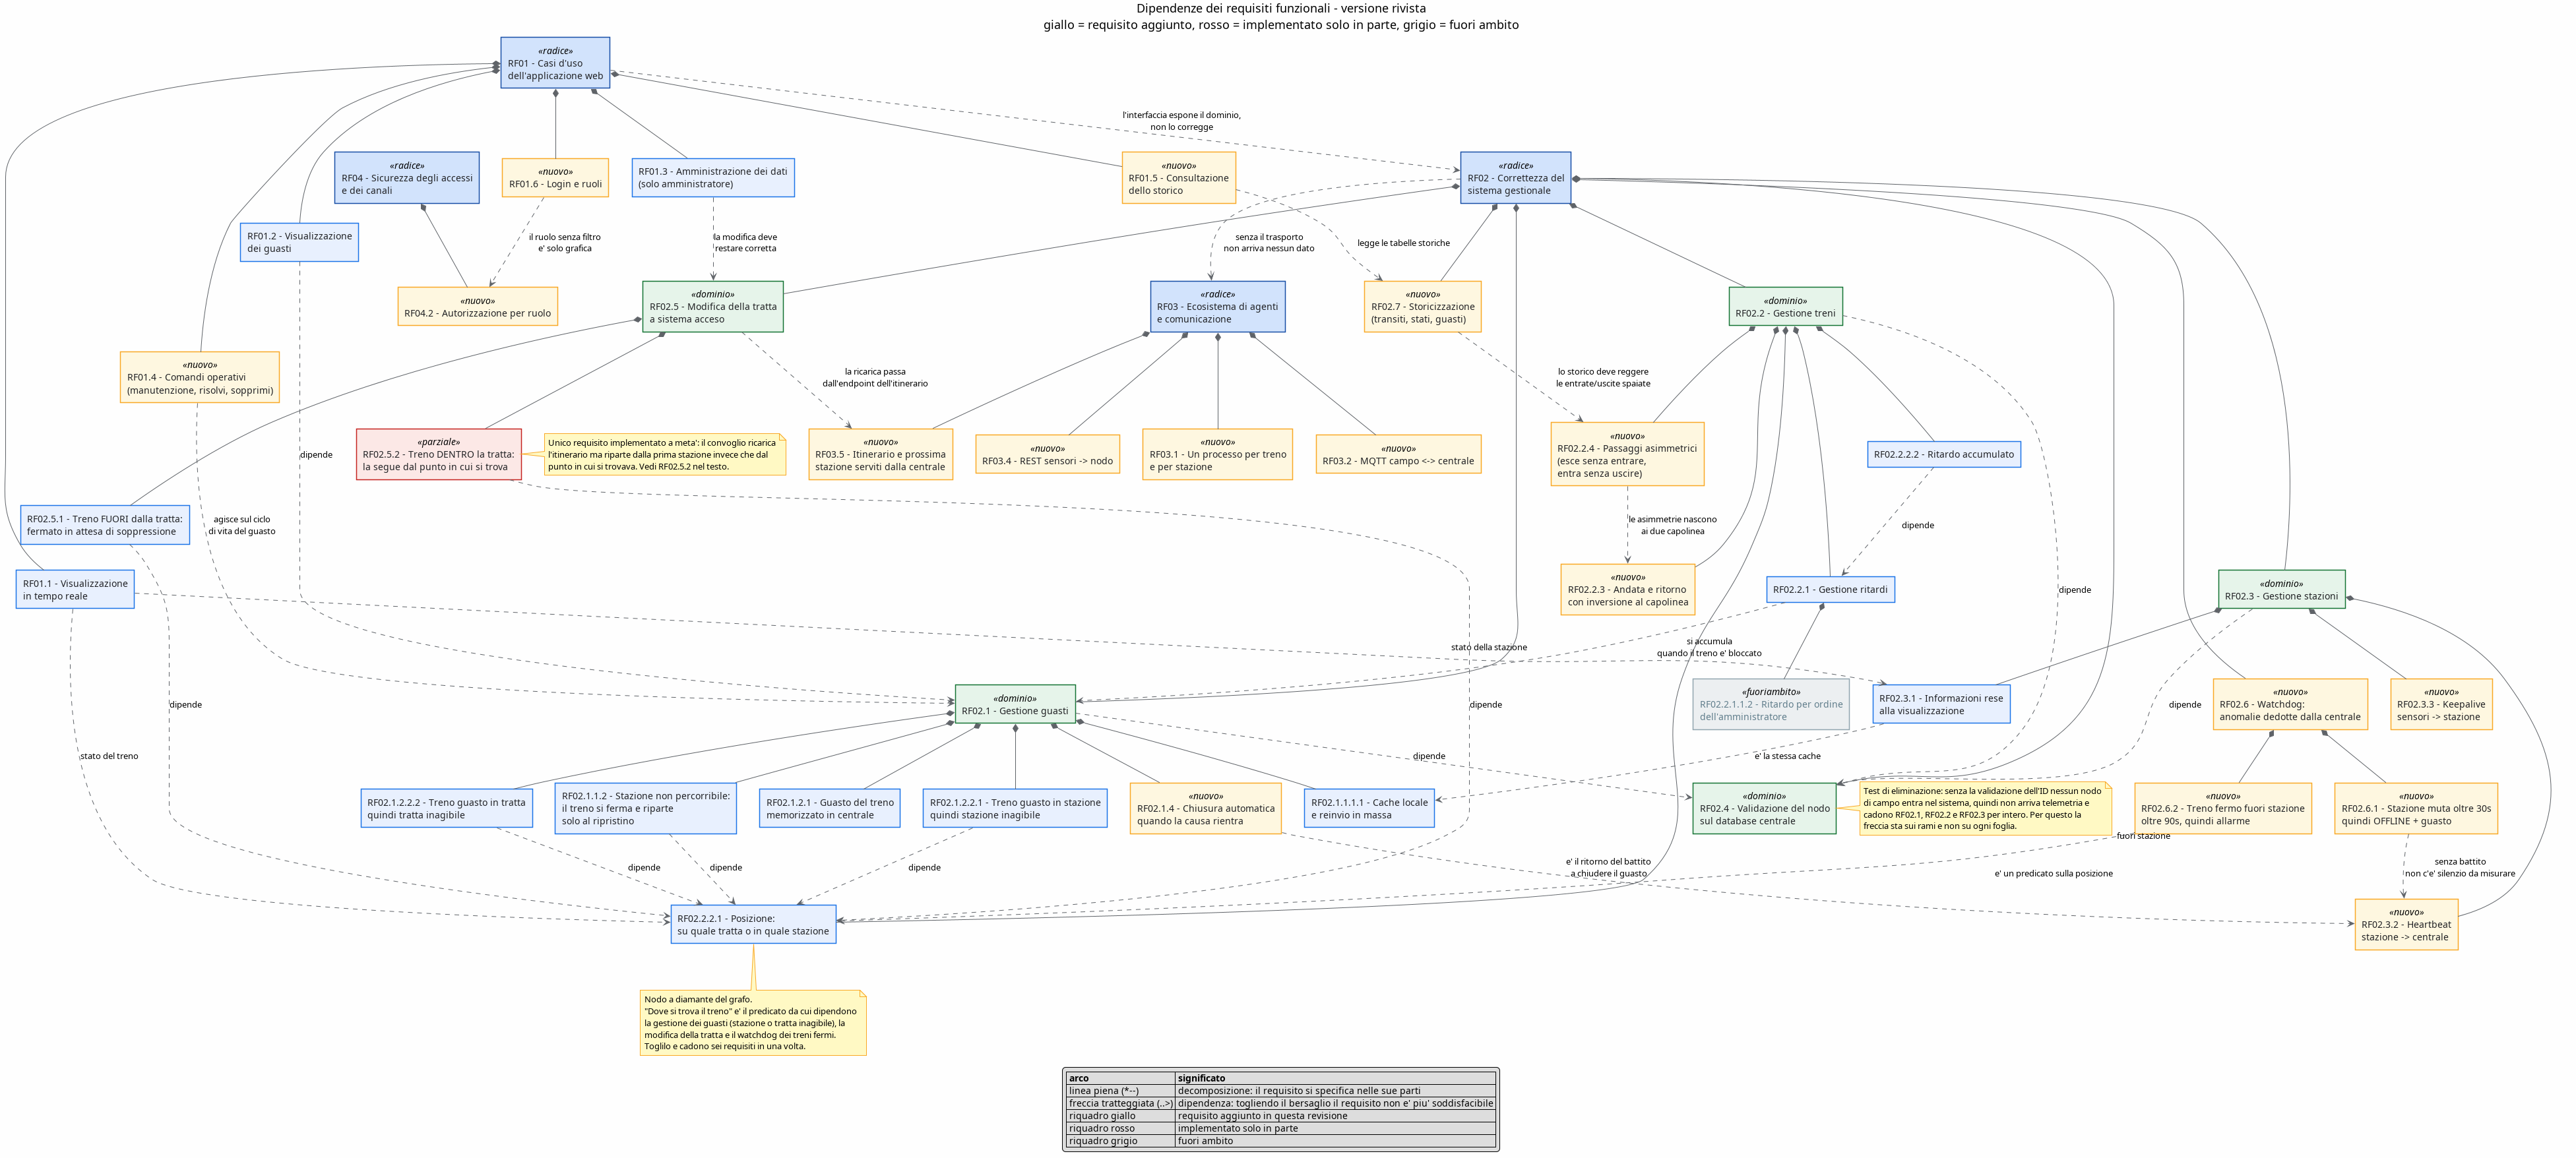
\includegraphics[width=.9\linewidth]{rf_grafo_dipendenze_aggiornato.png}
\label{}
\end{center}
\section{Matrice di tracciabilita'}
\label{sec:org25d1018}

Serve per la domanda ``dove sta questo requisito nel codice?'', che e' quella che rischia di arrivare
per prima.

\begin{center}
\begin{tabular}{llll}
RF & requisito (in breve) & macchine & codice principale\\
\hline
RF01.1.1 & mappa del traffico & M3, M11 & \texttt{TrafficMapPage.tsx}, \texttt{RealtimeWebSocket}\\
RF01.1.2 & elenco treni & T8, M3, M13 & \texttt{GET /api/treni}, \texttt{TrainsPage.tsx}\\
RF01.1.3 & elenco stazioni & S11, M12 & \texttt{GET /api/stazioni}, \texttt{StationsPage.tsx}\\
RF01.1.4 & push realtime & M11 & \texttt{/ws/realtime}, \texttt{websocketClient.ts}\\
RF01.1.5 & KPI di sintesi & M10 & \texttt{TrafficLogicEngine.kpiDashboard}\\
RF01.2 & allarmi & M6, M7, M8 & \texttt{GET /api/allarmi}, \texttt{AlertsPage.tsx}\\
RF01.3 & CRUD anagrafica & M10 & \texttt{RestApiGateway}, \texttt{components/admin/*}\\
RF01.4.1 & invio manutenzione & M10, S9 & \texttt{POST /api/stazioni/\{id\}/manutenzione}\\
RF01.4.2 & risoluzione allarme & M7, M10, T9 & \texttt{POST /api/allarmi/\{id\}/risolvi}\\
RF01.4.3 & soppressione treno & M10, T9, T6 & \texttt{POST /api/treni/\{id\}/sopprimi}\\
RF01.5 & storico transiti & M5 & \texttt{GET /api/transiti}, \texttt{StoricoTransito}\\
RF01.6 & login / sessione & M9 & \texttt{AuthController}, \texttt{SessioniAttive}\\
RF02.1.1.1 & cache e reinvio & S4, S5, S7 & \texttt{LocalBuffer}\\
RF02.1.1.2 & stazione non percorribile & T9, T11, T5 & \texttt{TrainGateway.riceviAlert}, \texttt{TrainJourneyEngine}\\
RF02.1.2 & guasto del treno e conseguenze & T10, M6, M7 & \texttt{TrainIngestion}, \texttt{IngestionService.onAlert}\\
RF02.1.4 & chiusura automatica & M4 & \texttt{IngestionService.onHeartbeat}\\
RF02.2.1 & ritardi & T5 & \texttt{TrainJourneyEngine}\\
RF02.2.2 & posizione e stato & T5, T6, T8 & \texttt{TrainDB}, \texttt{TrainElab}\\
RF02.2.3 & andata e ritorno & T7 & \texttt{TrainJourneyEngine} (inversione al capolinea)\\
RF02.2.4 & passaggi asimmetrici & T7, M5 & \texttt{TrainJourneyEngine.avviaViaggio}\\
RF02.3.1 & info della stazione & S8, S11 & \texttt{StationGateway}, \texttt{GET /stazione/treni}\\
RF02.3.2 & heartbeat stazione & S3, M4 & \texttt{HeartbeatGenerator}\\
RF02.3.3 & keepalive sensori & S6, S7, S10 & \texttt{POST /stazione/sensore/heartbeat}, \texttt{HeartbeatGenerator.manutenzionePeriodica}\\
RF02.4 & validazione del nodo & T2, S2, M2 & \texttt{TrainDatabaseValidator}, \texttt{ExistIdForEdge}\\
RF02.5 & modifica della tratta & M10, T9, T3 & \texttt{RestApiGateway.updateTratta}\\
RF02.6 & watchdog & M8 & \texttt{FaultMonitor}\\
RF02.7 & storicizzazione & M3, M5, M7 & entita' \texttt{Storico*}\\
RF03.1 & ecosistema di agenti & T1, S1, M1 & moduli \texttt{Treni} e \texttt{Stazioni}, N istanze\\
RF03.2 & topic MQTT & tutte & \texttt{application.properties} dei tre moduli\\
RF03.4 & REST dei sensori & S6, T10 & \texttt{StationIngestion}, \texttt{TrainIngestion}\\
RF03.5 & itinerario e prossima stazione & T3, M10 & \texttt{GET /api/treni/\{id\}/itinerario}, \texttt{/api/prossima-stazione}\\
RF04.2 & autorizzazione per ruolo & M9 & \texttt{FiltroAutorizzazione}\\
RF04.3 & TLS & - & profilo \texttt{\%tls}, \texttt{BrokerMosquitto/tls/gen-certs.sh}\\
\end{tabular}
\end{center}
\section{Riepilogo di cio' che e' dichiarato non fatto}
\label{sec:orgb38aa1e}

Tenerlo in un elenco unico e corto conviene: sono le cose su cui vale la pena avere una risposta
pronta invece di scoprirle davanti al prof.

\begin{center}
\begin{tabular}{lll}
requisito & stato & perche'\\
\hline
RF02.5.2 & \texttt{PARZIALE} & dopo la modifica della tratta il convoglio ricarica ma riparte dalla prima stazione; la correzione e' descritta nel requisito\\
RF02.2.1.1.2 & \texttt{FUORI AMBITO} & non esiste un comando ``rallenta questo treno'': non e' chiesto dal PDF e non l'ho implementato\\
previsione dell'orario di arrivo & \texttt{FUORI AMBITO} & il PDF cita ``previsioni di arrivo'' accanto al calcolo dei ritardi; il sistema calcola e mostra il ritardo corrente, non una stima dell'arrivo futuro (l'ETA che compare in \texttt{StationsPage} e' l'orario dichiarato, non una previsione)\\
vie multiple in stazione & \texttt{FUORI AMBITO} & il PDF la mette come opzione (``se volete gestire anche le vie multiple''). La stazione ha il campo \texttt{binari} ma non c'e' assegnazione del binario al singolo convoglio\\
\end{tabular}
\end{center}
\section{Nota sui file vicini}
\label{sec:org672585e}

\begin{itemize}
\item \texttt{00\_grafo\_dipendenze\_requisiti.puml} disegna la lista \textbf{vecchia}: e' superato dal grafo di questo
file e va tenuto solo come storia della revisione, oppure riallineato.
\item La sezione ``Elenco maggiomente formale dei requisiti'' della documentazione finale puo' essere
sostituita da un rimando a questo file, cosi' non ci sono due liste che dicono cose diverse.
\end{itemize}
\end{document}
